\section{Trace Funktion}\label{Validierung:Trace Funktion}
\begin{itemize}
  \item Beispielprogramme in PEARL definieren
  \item Anforderungen validieren:
  \begin{itemize}
    \item Laufzeiten der einzelnen Programme mit und ohne Trace Funktionalität
    bestimmen und vergleichen, mit Python Programm
    \cref{lst:Python_Benchmark_CPU}
    \item Speicherauslastung der einzelnen Programme mit und ohne Trace
    Funktionalität bestimmen und vergleichen, mit Python Programm
    \cref{lst:Python_Benchmark_Memory}
  \end{itemize}
\end{itemize}

\begin{listing}[ht]
  \inputminted[frame=lines,linenos]{python}{./Python/benchmark_cpu.py}
  \caption{Pythonskipt zur Messung der Laufzeit}
  \label{lst:Python_Benchmark_CPU}   
\end{listing} 

\begin{listing}[ht]
  \inputminted[frame=lines,linenos]{python}{./Python/benchmark_memory.py}
  \caption{Pythonskipt zur Messung der Speicherauslastung}
  \label{lst:Python_Benchmark_Memory}   
\end{listing} 

\section{Analyse Programm}
\label{section:ValidierungAnalyseProgramm}
Für die chronologische Darstellung der Lockobjekte wird die Trace-Datei aus
\cref{lst:ExampleTraceFile} mit drei Threads, neun Lockobjekten und einem
potenziellen Deadlock verwendet.
\begin{listing}[ht]
  \begin{minipage}[ht]{\linewidth}
    \begin{multicols}{3}
      \inputminted[linenos]{vim}{./Examples/ExampleTraceFile.log}
    \end{multicols}
    \caption{Beispielhafte Trace-Datei mit einem potenziellen Deadlock}
    \label{lst:ExampleTraceFile}
  \end{minipage}
\end{listing}
In dem Beispiel gibt es zusätzlich zwei Einträge mit dem gleichen Zeitstempel in
den Zeilen 3 und 4 sowie in den Zeilen 13 und 14. Die Ausgabe der Anwendung aus
\cref{section:Implementierung:Analyse Programm} ist in
\cref{fig:LockTraceVisualization} dargestellt.
\begin{figure}[ht]
  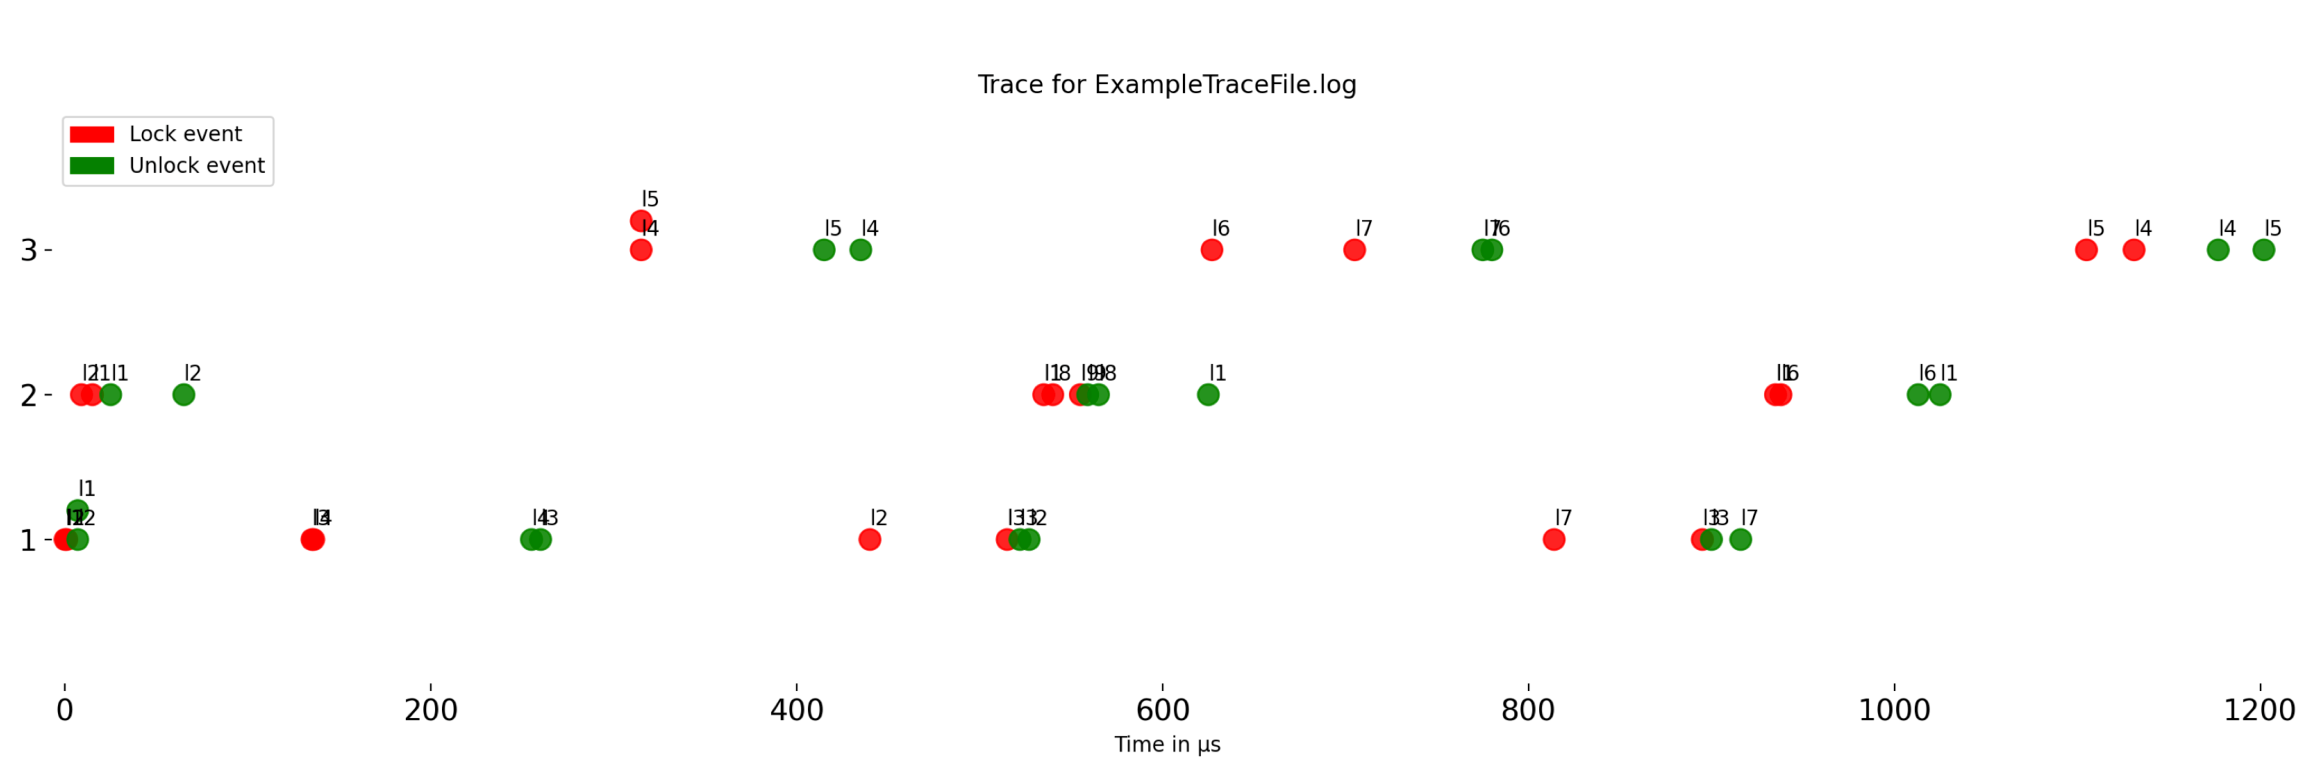
\includegraphics[width=\linewidth]{ExampleTraceFile.eps}
  \caption{Ausgabe der Analyse-Anwendung}
  \label{fig:LockTraceVisualization}
\end{figure}
Die überlappenden Logeinträge können auseinander gezogen werden in dem in den
Graphen hineingezoomt wird. Wird zum Beispiel auf die ersten 70 Mikrosekunden
vergrößert, werden die Logeinträge auseinander gezogen siehe
\cref{fig:LockTraceVisualizationZoomed}.
\begin{figure}[ht]
  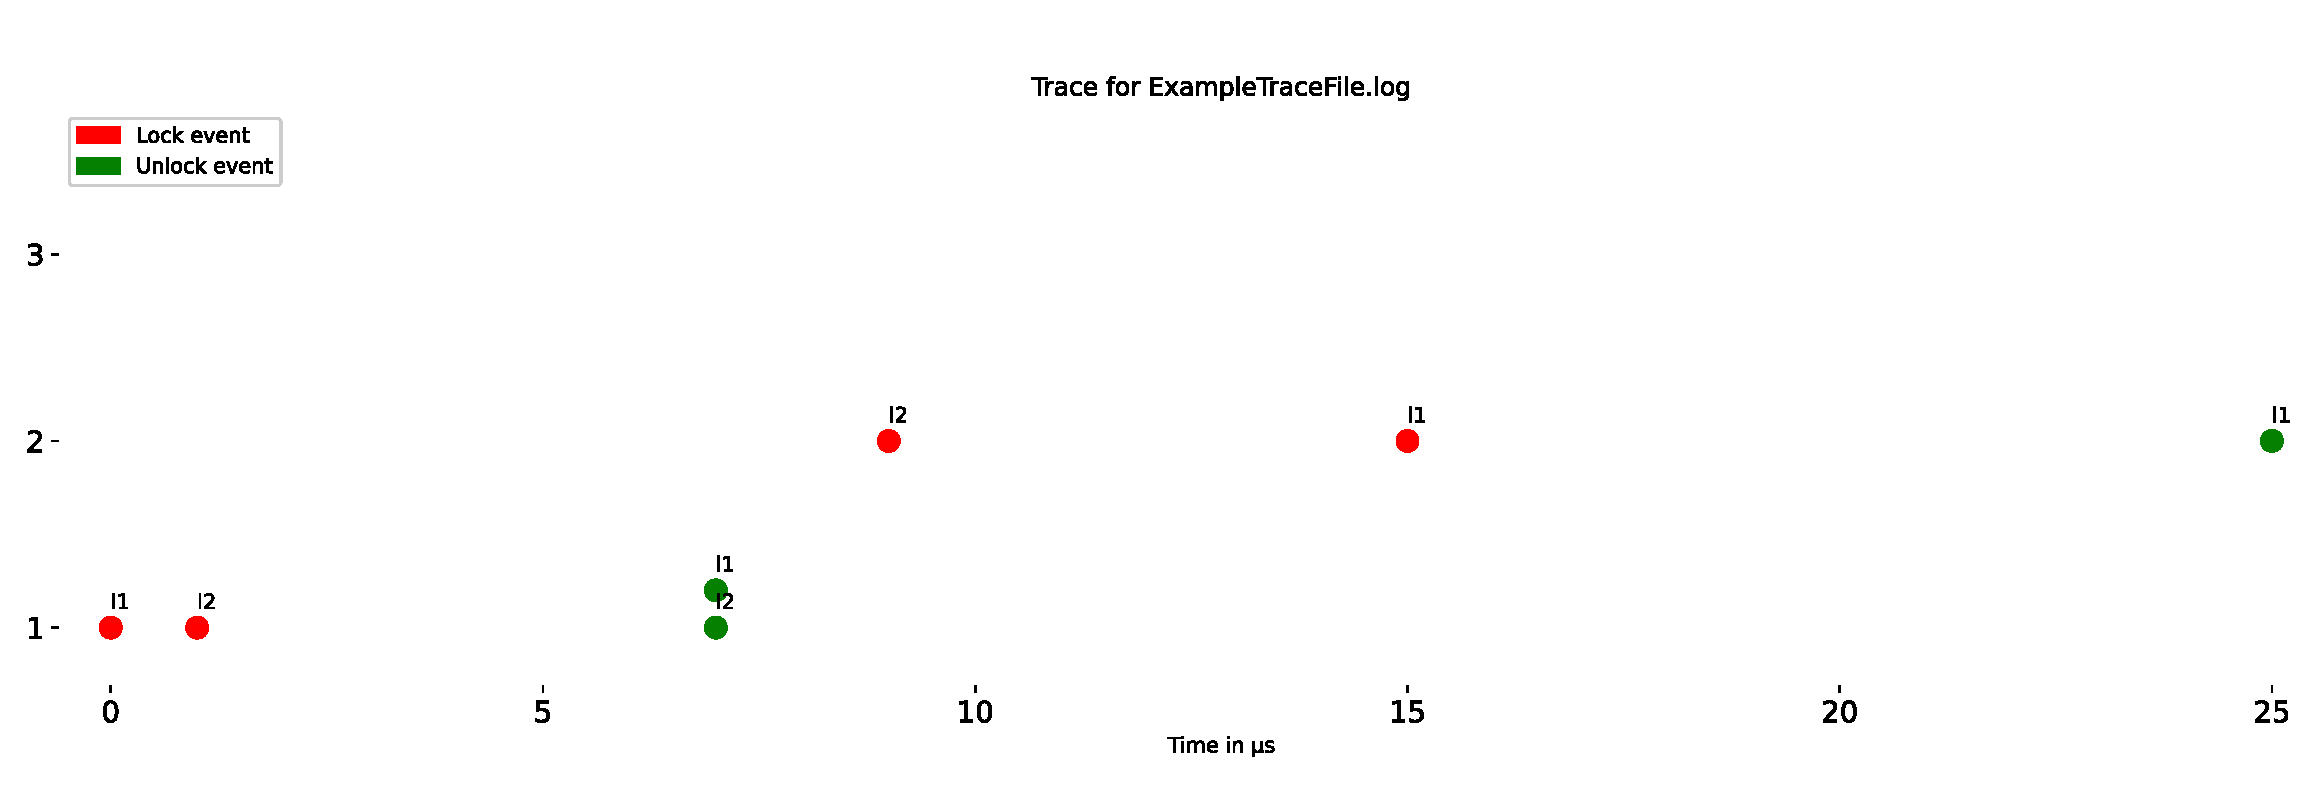
\includegraphics[width=\linewidth]{ExampleTraceFileZoomed.eps}
  \caption{Vergrößerte Darstellung von \cref{fig:LockTraceVisualization}}
  \label{fig:LockTraceVisualizationZoomed}
\end{figure}
Die beiden Logeinträge mit den gleichen Zeitstempel sind bei 7 Mikrosekunden
korrekt vertikal versetzt dargestellt.


\section{Visualisierung von potenziellen Deadlocks}
\begin{itemize}
  \item Die aus \cref{Validierung:Trace Funktion} erstellten Trace-Dateien
  auswerten und die potenziellen Deadlocks visuell als gerichtete Graphen
  aufzeigen
\end{itemize}